\chapter{The Bornholdt model}\label{ch:bornholdt_model}
In the spirit of finding a model for the price dynamics of risky assets, we now present the model proposed in \cite{bornholdt}. The idea is to formulate a model with maximum simplicity, which includes the possibility of strategic interaction between agents in the market.



\section{Introduction}
\subsection{Financial motivation}
In \cite{bornholdt}, a simple spin model, which we will refer to as the Bornholdt model, is proposed to model trading in financial markets. In the model, agents are seen as interacting spins, which have two possible actions: buy or sell an asset. The choice of each agent is influenced by two contrasting forces:
\begin{itemize}
    \item ``Do what your neighbors do'': this is the strategy that momentum traders follow. They try to follow the trend in the market, buying when the price is rising and selling when it is falling.
    \item ``Do what the minority does'': this is the strategy that mean-reversion traders follow. They try to buy when the price is falling and sell when it is rising, betting on a reversal of the trend.
\end{itemize}
We will see how these two strategies are implemented in the model.

\subsection{Model definition}
Consider a model with N spins with orientations $\sigma_i\in\{-1,+1\}$, representing the decision of agent $i$ to buy or sell a stock. We will consider updates following a heat-bath dynamics:
\begin{equation}
    \begin{aligned}
        \sigma_i(t+1) &= +1 \;\text{with }\; p = \frac{1}{1+e^{-2\beta h_i(t)}}\\
        \sigma_i(t+1) &= -1 \;\text{with }\; 1-p
    \end{aligned}
    \label{eq:heat_bath}
\end{equation}
Where $h_i(t)$ is the local field of agent $i$ at time $t$:
\begin{equation}
    h_i(t)=\sum_{j=1}^N J_{i j} \sigma_j-\alpha C_i(t) \frac{1}{N} \sum_{j=1}^N \sigma_j(t)
\end{equation}
Where $J_{i j}$ is the coupling between agents $i$ and $j$, $\sigma_j$ is the agent's action at $t$, $C_i(t)$ is the strategy of $i$ at time $t$, and $\alpha$ is a parameter. The first term in the local field pushes the agent to follow the trend of spins in their proximity (do what your neighbors do), while the second term pushes the agent to follow the minority (do what the minority does), assuming the strategy $C_i(t)$ is positive. 
If we consider the case in which $C_i(t) = 1\;\forall i, t$, we have that each trader follows both a momentum and a mean-reversion strategy simultaneously. This leads to near-vanishing magnetization even for temperatures below the critical temperature. 
We will focus on the more interesting and realistic case in which the strategies are updated at each time by each agent. Specifically, we will assume that a trader in the majority will try to switch to the minority strategy and thus adopt $C_i(t+1) = +1$, while a trader in the minority will try to switch to the majority strategy and thus adopt $C_i(t+1) = -1$. This is a reasonable assumption, as traders in the minority are likely to be more cautious and risk-averse, while traders in the majority are likely to be more aggressive and willing to take risks. This dynamics is the described by:
\begin{equation}
    C_i(t+1) = \begin{cases}
        +1 & \text{if} \quad \alpha\sigma_i(t) \sum_{j=1}^N \sigma_j(t)> 0\\
        -1 & \text{otherwise}
    \end{cases}
\end{equation}
Rearranging the equation, we can write:
\begin{equation}
    C_i(t+1) = \begin{cases}
        +C_i(t) & \text{if} \quad \alpha\sigma_i(t)C_i(t) \sum_{j=1}^N \sigma_j(t)> 0\\
        -C_i(t) & \text{otherwise}
    \end{cases}
\end{equation}
Now, we can take one extra step and assume that the strategy update is done instantaneously, so that we can write:
\begin{equation}
    C_i(t) = \begin{cases}
        +C_i(t) & \text{if} \quad \alpha\sigma_i(t)C_i(t) \sum_{j=1}^N \sigma_j(t)> 0\\
        -C_i(t) & \text{otherwise}
    \end{cases}
\end{equation}
Then, substituting this into the local field, we have a remarkably simple expression for the local field:
\begin{equation}
    h_i=\sum_{j=1}^N J_{i j} \sigma_j-\alpha \sigma_i \left | \frac{1}{N}\sum_{j=1}^N \sigma_j \right |
\end{equation}
Then, the hamiltonian of the model is:
\begin{equation}
    \begin{aligned}
        H(\underline{\sigma}) &= -\sum_{i=1}^N \sigma_i h_i\\
        &= -\sum_{i,j}J_{i,j}\sigma_i\sigma_j + \frac{\alpha}{N}\sum_{i=1}^N \sigma_i \left | \sum_{j=1}^N \sigma_j \right |
    \end{aligned}
\end{equation}
At this point, the magnetization \(M = \frac{1}{N}\sum_{j=1}^N \sigma_j\) can be interpreted as the price of the security that is being traded. We seek to study the dynamics of the model.

\subsection{Analysis of the model}
We will focus on the fully connected case in which \(J_{i,j}=\frac{J}{N} \; \forall i,j\). The hamiltonian of the model is then:
\begin{equation}
    H(\underline{\sigma}) = -\frac{J}{N}\sum_{i,j}\sigma_i\sigma_j + \frac{\alpha}{N}\sum_{i=1}^N \sigma_i \left | \sum_{j=1}^N \sigma_j \right |
\end{equation}

We will proceed in a similar way as in Section~\ref{sec:curie_weiss}, by introducing a combinatorial factor $\mathcal{N}(m)$ and taking the large $N$ limit.

The partition function of the model is given by:
\begin{equation}
    \begin{aligned}
        Z &= \sum_{\underline{\sigma}\in\mathcal{X}_N}e^{-\beta H(\underline{\sigma})}\\
        &= \sum_{\underline{\sigma}\in\mathcal{X}_N}e^{-\beta\frac{J}{N}\sum_{i,j}\sigma_i\sigma_j + \beta\frac{\alpha}{N}\sum_{i=1}^N \sigma_i \left | \sum_{j=1}^N \sigma_j \right |}\\
        &= \sum_{\underline{\sigma}\in\mathcal{X}_N}e^{-\beta\frac{J}{N}\left(\sum_{i}\sigma_i\right)^2 + \beta\frac{\alpha}{N}\sum_{i=1}^N \sigma_i \left | \sum_{j=1}^N \sigma_j \right |}\\
    \end{aligned}
\end{equation}
Now, we can introduce the notation:
\begin{equation}
m(\underline{\sigma}) = \frac{1}{N}\sum_{i}\sigma_i
\end{equation}
Then, we can rewrite the hamiltonian as:

\begin{equation}
    H(\underline{\sigma}) =  - J N m^2(\underline{\sigma}) + \alpha N m(\underline{\sigma}) \left| m(\underline{\sigma}) \right|
\end{equation}

And the partition function becomes:
\begin{equation}
    \begin{aligned}
        Z &= \sum_{\underline{\sigma}\in\mathcal{X}_N}e^{N\left(\beta J  m^2(\underline{\sigma})+\beta \alpha  m(\underline{\sigma}) \left| m(\underline{\sigma})\right|\right)}\\
        &= \sum_{m}e^{N\left(\beta J  m^2+\beta \alpha  m \left| m\right|\right)}\mathcal{N}(m)\\
        &= \sum_{m}e^{N\left(\beta J  m^2+\beta \alpha  m \left| m\right| + \frac{1}{N}\log \mathcal{N}(m)\right)}\\
    \end{aligned}
\end{equation}
Where $\mathcal{N}(m)$ is the number of configurations with magnetization $m$. In Section~\ref{sec:curie_weiss}, we have seen that $S(m) :=\lim_{N\rightarrow\infty}\frac{1}{N}\log \mathcal{N}(m)$ is the Shannon entropy of a bernoulli distribution with probability $p = \frac{1+m}{2}$ and $q = \frac{1-m}{2}$.

Then, in the large $N$ limit, we notice the following:
\begin{itemize}
    \item The increments of $m$ become infinitesimal, allowing us to treat the sum as an integral.
    \item We can subtitute $\frac{1}{N}\log\mathcal{N}(m)$ with $S(m)$.
\end{itemize}
Then, we can rewrite the partition function as:
\begin{equation}
    Z \approx \int_{-1}^{1} dm e^{N\phi(m)}, \quad \text{where }
    \phi(m) = \beta J m^2 + \alpha m |m| + S(m)
    \label{eq:bornholdt_phi}
\end{equation}


We now aim to rewrite $\phi(m)$ in a more convenient form. First, we notice that:
\begin{equation}
    x|x| = x^2 (2\theta(x)-1)
\end{equation}
Where $\theta(x)$ is the Heaviside step function:
\begin{equation}
    \theta(x) = \begin{cases}
        0 & \text{if } x < 0\\
        1 & \text{if } x \geq 0
    \end{cases}
\end{equation}
Which we can write as:
\begin{equation}
    \theta(x) = \int_{-\infty}^{x} \delta(t) dt
\end{equation}
Then, we can rewrite $\phi(m)$ as:
\begin{equation}
    \phi(m) = \beta J m^2 + \alpha m^2 (2\theta(m)-1) + S(m)
\end{equation}
Without going into the technical details, writing $\phi(m)$ in this way allows us to take its weak derivative and obtain the saddle point equation:
\begin{equation}
    \begin{gathered}
        \frac{d \phi(m)}{d m} = 0\\
        \implies 2\beta J m - 2 \alpha \beta m^2 \delta(m) - 4 \alpha \beta m \theta(m) + 2\alpha \beta m + \frac{1}{2} \log \frac{1-m}{1+m} = 0\\
        \implies 2\beta J m - 4 \alpha \beta m \theta(m) + 2\alpha \beta m = \arctanh(m)\\
    \end{gathered}
\end{equation}
From which we get the self-consistent equation:
\begin{equation}
    m = \tanh\left(2\beta J m - 4 \alpha \beta m \theta(m) + 2\alpha \beta m\right)
    \label{eq:bornholdt_self_consistent}
\end{equation}

\begin{figure}[h]
    \centering
    \begin{minipage}[t]{0.45\textwidth}
        \centering
        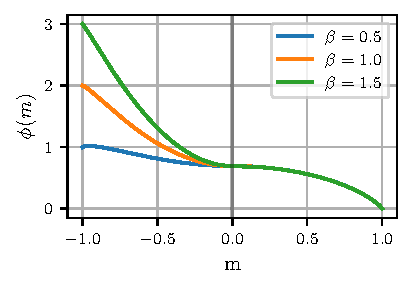
\includegraphics[width=\textwidth]{bornholdt/bornholdt_phi.pdf}
    \end{minipage}
    \hfill
    \begin{minipage}[t]{0.45\textwidth}
        \centering
        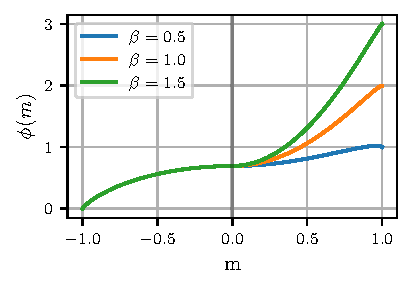
\includegraphics[width=\textwidth]{bornholdt/bornholdt_phi_negative_alpha.pdf}
    \end{minipage}
    \caption{The function $\phi(m)$ defined in Equation~\ref{eq:bornholdt_phi} for different values of $\beta$, with $J=1$ and $\alpha=1$ (left) and $\alpha=-1$ (right).}
    \label{fig:bornholdt_phi}
\end{figure}

\begin{figure}[h]
    \centering
    \begin{minipage}[t]{0.45\textwidth}
        \centering
        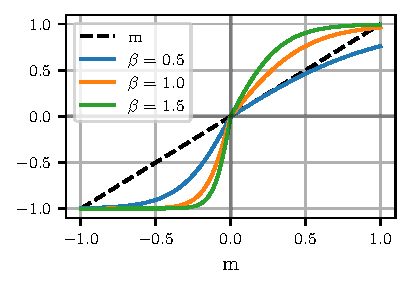
\includegraphics[width=\textwidth]{bornholdt/bornholdt_rhs_lhs.pdf}

    \end{minipage}
    \hfill
    \begin{minipage}[t]{0.45\textwidth}
        \centering
        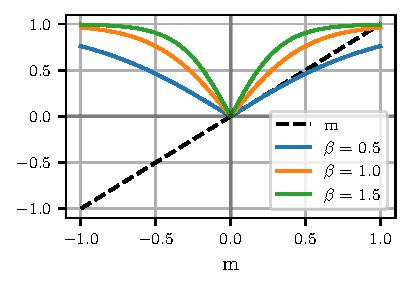
\includegraphics[width=\textwidth]{bornholdt/bornholdt_rhs_lhs_negative_alpha.pdf}
    \end{minipage}
    \caption{The left-hand side and right-hand side of Equation~\ref{eq:bornholdt_self_consistent} for $J=1$ and $\alpha=1$ (left) and $\alpha=-1$ (right). Intersecting points correspond to solutions of the equation.}
    \label{fig:bornholdt_rhs_lhs}
\end{figure}

\section{Simulations of the Bornholdt model}
We conducted a numerical simulation of the Bornholdt model, employing a system consisting of 1024 spins arranged in a two-dimensional square lattice. The coupling constant was set to $J=1.0$, the external field parameter was $\alpha=4.0$, and the temperature of the system was defined as $T=1/\beta=1.5$. The simulation was carried out over a sufficiently large number of time steps to allow the results to be representative of the model's long-term dynamics.

\subsection{Only fundamental traders}
We start by analysing the case in which all agents are fundamental traders, meaning that they all follow the same strategy. In this case, we set $C_i(t) = 1$ for all agents and all times. The results of the simulation are shown in figure \ref{fig:fundamental_traders}. As expected, the system is stuck in a noisy state in which the magnetization fluctuates between low positive and negative values.

\begin{figure}[H]
    \centering
    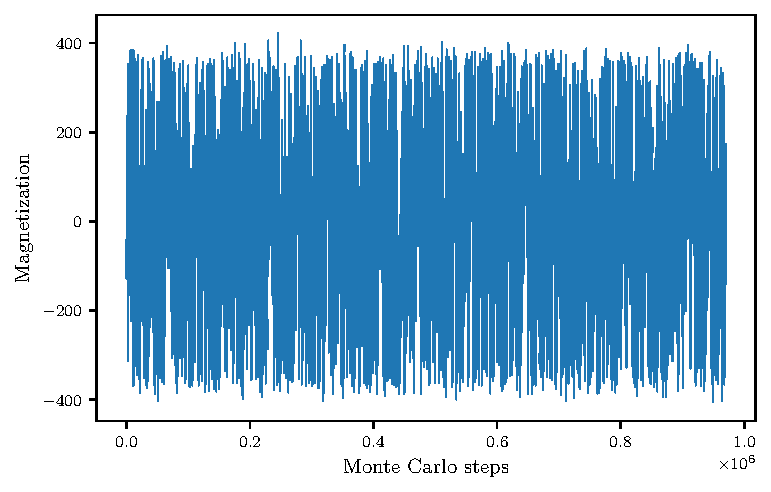
\includegraphics[width=0.9\textwidth]{constant_c_magnetization.pdf}
    \caption{Dynamics of the magnetization of the system with only fundamental traders.}
    \label{fig:fundamental_traders}
\end{figure}

\subsection{Dynamics of the strategies}
The simulations indicate that the initial distribution of agents' strategies has a negligible long-term impact on the system's behavior. Regardless of the starting configuration, the system quickly converges to a stable state where approximately 50\% to 70\% of agents adopt the strategy $C_i(t) = 1$. This convergence is evident from the dynamics shown in figure \ref{fig:strategies}. Consequently, for the purposes of simulating the model, it is not necessary to distinguish between different initial distributions of strategies, as the system's evolution is largely independent of these initial conditions.

\begin{figure}[H]
    \centering
    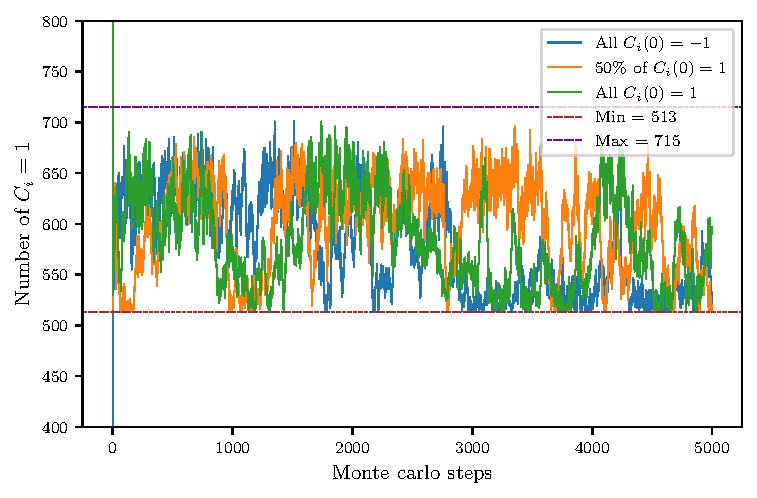
\includegraphics[width=0.9\textwidth]{c_values.pdf}
    \caption{Dynamics of agent's strategy based on different starting distributions.}
    \label{fig:strategies}
\end{figure}

\subsection{Dynamics of the price}
Following the interpretation proposed in \cite{bornholdt}, the magnetization of the system is treated as the price of a financial asset being traded by the agents. By plotting the magnetization as a function of time, we obtain a time-series that mimics the price dynamics of a financial asset. This is illustrated in figure \ref{fig:magnetization}, where the temporal evolution of the magnetization is shown.

In addition to examining the magnetization (i.e., the price), it is also insightful to analyze the underlying configuration of spins that produces this magnetization. The spin configuration provides a microscopic view of the system's state, which complements the macroscopic perspective offered by the magnetization. As shown in figure \ref{fig:lattices}, the system alternates between two distinct regimes: metastable states, where the spin configuration remains relatively stable over time, and turbulent states, characterized by rapid and chaotic changes in the spin configuration. These alternating regimes highlight the complex dynamics of the system and their influence on the observed price behavior.

\begin{figure}[H]
    \centering
    \includegraphics[width=0.9\textwidth]{magnetization.pdf}
    \caption{Dynamics of the magnetization of the system.}
    \label{fig:magnetization}
\end{figure}

\begin{figure}[H]
    \centering
    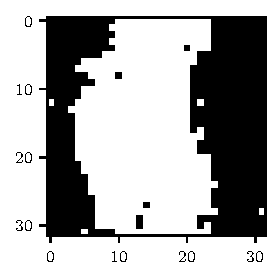
\includegraphics[width=0.3\textwidth]{lattices/metastable_turbulent/43400.pdf}
    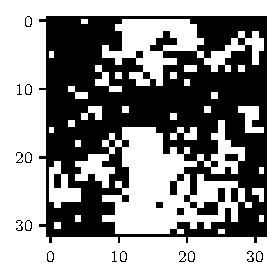
\includegraphics[width=0.3\textwidth]{lattices/metastable_turbulent/43700.pdf}
    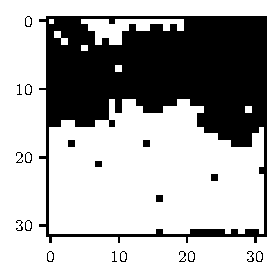
\includegraphics[width=0.3\textwidth]{lattices/metastable_turbulent/43850.pdf}
    \caption{Snapshots of the lattices at times $t=43400$, $t=43700$ and $t=43850$.}
    \label{fig:lattices}
\end{figure}

\subsection{Dynamics and statistical properties of the returns}
To analyze the dynamics of the returns of the asset, we define the log-returns as the logarithm of the ratio of the magnetization at consecutive time steps. Since the magnetization $M(t)$ can take on both positive and negative values, we use its absolute value to ensure that the log-returns are well-defined. Additionally, to avoid issues with division by zero or taking the logarithm of zero, we introduce a small positive constant $\epsilon$, where $\epsilon \ll 1$. The log-returns are then computed as:
\begin{equation}
    R(t) = \log\left(\frac{|M(t)| + \epsilon}{|M(t-1)| + \epsilon}\right)
\end{equation}
Here, $R(t)$ represents the return at time $t$, $M(t)$ is the magnetization at time $t$, and $\epsilon$ is a small constant added for numerical stability.

The resulting time-series of the returns is shown in figure \ref{fig:returns}.

\begin{figure}[H]
    \centering
    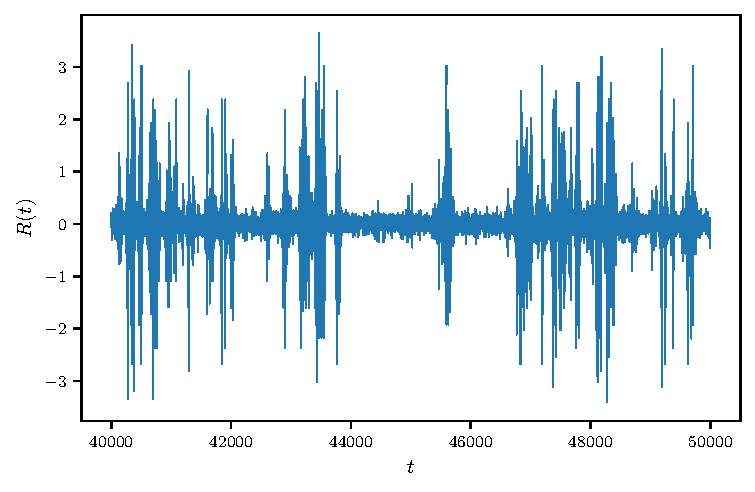
\includegraphics[width=0.9\textwidth]{returns.pdf}
    \caption{Time-series of the returns of the asset.}
    \label{fig:returns}
\end{figure}

From a financial perspective, we are interested in checking wether the returns exhibit the statistical properties of real financial data, namely fat tails and autocorrelation, as noted in \cite{bouchaud2000theory}.

\subsubsection{Fat tails}
The analysis of the distribution of the returns, as illustrated in figures \ref{fig:returns_distribution} and \ref{fig:cumulative_returns_distribution}, provides strong evidence that the returns exhibit fat tails. This characteristic is a hallmark of financial time-series and indicates that extreme events (large positive or negative returns) occur more frequently than would be expected under a normal distribution.

To further investigate this property, we compare the returns to a normal distribution using a QQ-plot, shown in figure \ref{fig:qqplot}. The QQ-plot clearly demonstrates significant deviations from the straight line that would be expected if the returns were normally distributed. These deviations, particularly in the tails, confirm the presence of fat tails in the distribution.

Additionally, we perform a statistical test to formally assess whether the returns follow a normal distribution. Specifically, we use the Shapiro-Wilk test, which tests the null hypothesis that the data is drawn from a normal distribution. The results of the test yield a p-value on the order of $10^{-192}$. Such an extremely small p-value indicates that we can reject the null hypothesis with extremely high confidence, confirming that the returns are not normally distributed. Additionally, we compute the kurtosis of the returns, which is approximately 24.2. This value indicates an extremely leptokurtic distribution, suggesting a very high likelihood of outliers. \cite{kurtosis_skewness} shows that stocks in the Dow Jones Industrial Average show kurtosis values ranging from 1.08 to 24.13. This means we could see the price movements of the Bornholdt model as a very volatile stock.

\begin{figure}[H]
    \centering
    \begin{minipage}[T]{0.45\textwidth}
        \centering
        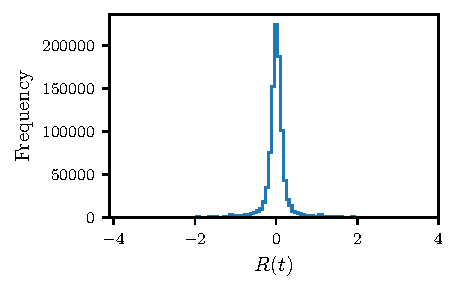
\includegraphics[width=\textwidth]{distribution_returns.pdf}
        \caption{Distribution of the returns of the asset.}
        \label{fig:returns_distribution}
    \end{minipage}
    \hfill
    \begin{minipage}[T]{0.45\textwidth}
        \centering
        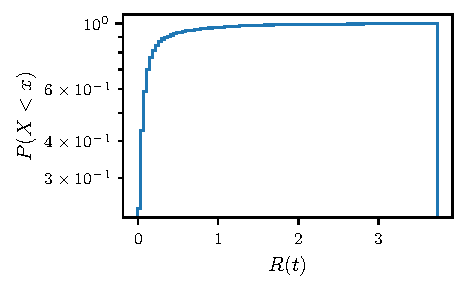
\includegraphics[width=\textwidth]{cumulative_distribution.pdf}
        \caption{Cumulative distribution of the returns of the asset.}
        \label{fig:cumulative_returns_distribution}
    \end{minipage}
\end{figure}


\subsubsection{Autocorrelation}
From figure \ref{fig:returns}, we can already seen that the periods of high volatility (i.e. large positive or negative returns) tend to be clustered together. This is a sign of autocorrelation in the returns. To quantify this, we can compute the autocorrelation function of the returns, defined as
\begin{equation}
    \rho(k) = \frac{\sum_{t=1}^{N-k} (R(t) - \bar{R})(R(t+k) - \bar{R})}{\sum_{t=1}^{N} (R(t) - \bar{R})^2}
\end{equation}
where $N$ is the number of returns, $R(t)$ is the return at time $t$, and $\bar{R}$ is the mean of the returns. The autocorrelation function measures the correlation between the returns at time $t$ and time $t+k$. A positive value of $\rho(k)$ indicates that the returns at time $t$ and time $t+k$ are positively correlated, while a negative value indicates that they are negatively correlated. A value close to zero indicates that there is no correlation between the returns at time $t$ and time $t+k$.
The autocorrelation function is computed for lags $k=1,2,\ldots,100$ and is shown in figure \ref{fig:autocorrelation}. The results show that the autocorrelation is significant for a large number of lags, which is consistent with the empirical observation that financial returns are autocorrelated.

\begin{figure}[H]
    \centering
    \begin{minipage}[T]{0.45\textwidth}
        \centering
        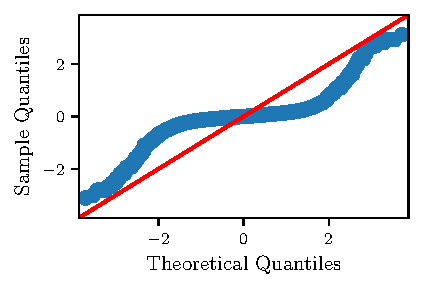
\includegraphics[width=\textwidth]{qqplot-returns.pdf}
        \caption{QQ-plot of the returns against a normal distribution.}
        \label{fig:qqplot}
    \end{minipage}
    \hfill
    \begin{minipage}[T]{0.45\textwidth}
        \centering
        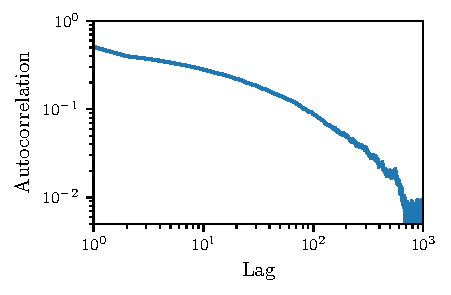
\includegraphics[width=\textwidth]{autocorrelation.pdf}
        \caption{Autocorrelation function of the returns.}
        \label{fig:autocorrelation}
    \end{minipage}
\end{figure}


\section{Discussion}
The results of the simulation suggest that the Bornholdt model is able to reproduce some of the statistical properties of real financial data, such as fat tails and autocorrelation of returns. This is interesting because the model is based on a simple spin model, and does not rely on any assumptions about the rationality of agents or the efficiency of markets.

As seen in \ref{sec:financial_background}, one of the main assumptions of the model introduced in \cite{black_scholes} is that the price of the underlying asset follows a geometric Brownian motion. The Bornholdt model, however, results in price dynamics which exhibit fat tails, and do not have independent increments, as shown by the autocorrelation of the returns, which is the case also in real financial data.

The key observation here is that, unlike in a geometric Brownian motion, the price (i.e. magnetization) at time $t$ is not enough to describe the distribution of prices at times $t+s, \; s\geq 0$. This might be counterintuitive, as by equation \ref{eq:heat_bath}, the future configuration of spins is determined by the current configuration of spins. However, it is important to note that the current magnetization is not enough to determine the current configuration of spins. In fact, the magnetization is a global property of the system, while the configuration can vary locally. In figures \ref{fig:lattices_m100} and \ref{fig:magnetization_m100}, we can see that the magnetization is the same at times $t=129722$ and $t=130293$, but the configuration of spins is completely different.

\begin{figure}[H]
    \centering
    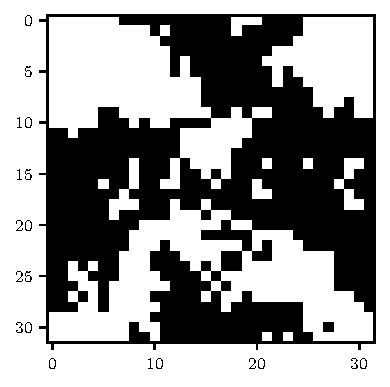
\includegraphics[width=0.4\textwidth]{lattices/same_magnetization/129722.pdf}
    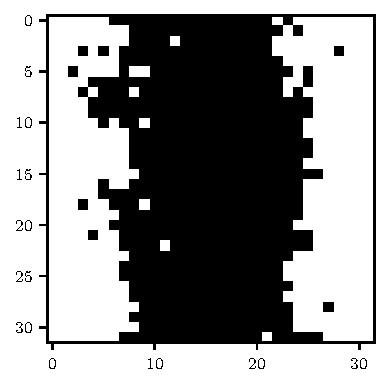
\includegraphics[width=0.4\textwidth]{lattices/same_magnetization/130293.pdf}
    \caption{Snapshots of the lattices at times $t=129722$, and $t=130293$.}
    \label{fig:lattices_m100}
\end{figure}

\begin{figure}[H]
    \centering
    \includegraphics[width=0.9\textwidth]{lattices/same_magnetization/magnetization.pdf}
    \caption{Dynamics of the magnetization of the system. The green lines represent the times at which the snapshots in figure \ref{fig:lattices_m100} were taken.}
    \label{fig:magnetization_m100}
\end{figure}